%    \begin{macrocode}
%</example-image-plain.tex>
%<*example-image-plain.tex&standalone>
\documentclass[border=0]{standalone}
\usepackage{tikz}
\begin{document}%
%</example-image-plain.tex&standalone>
%<*example-image-plain.tex>
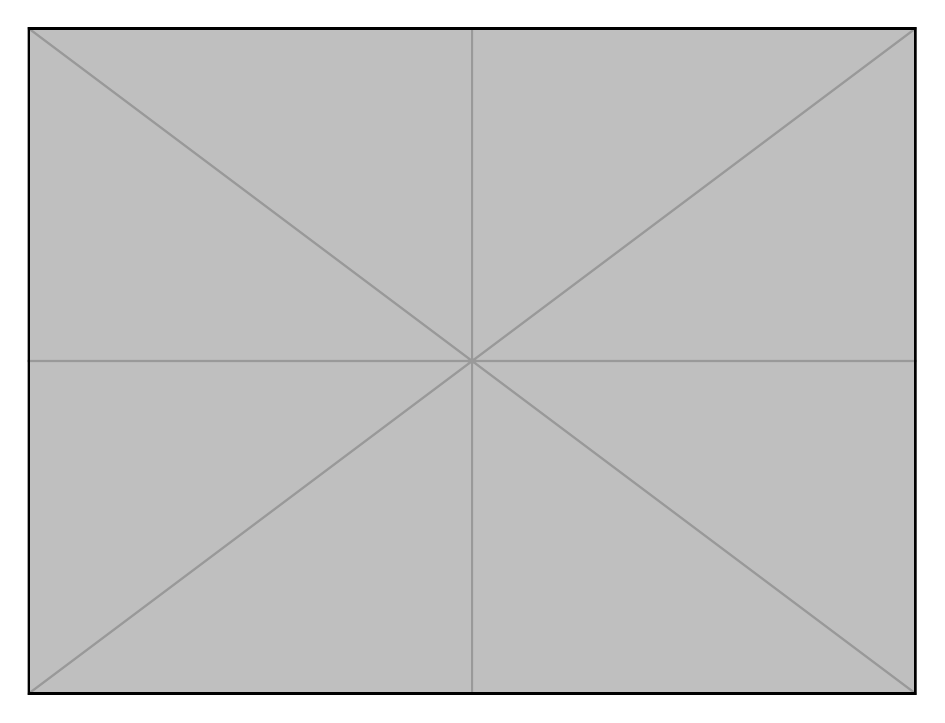
\begin{tikzpicture}[x=32bp,y=24bp]% 4x3
    \clip (0,0) rectangle (10,10);
    \path [fill=black!25] (0,0) rectangle (10,10);
    \draw [thick,black!40]
        (0,0) -- (10,10)
        (10,0) -- (0,10)
        (5,0) -- (5,10)
        (0,5) -- (10,5)
    ;
    \path [draw,ultra thick] (0,0) rectangle (10,10);
\end{tikzpicture}%
%</example-image-plain.tex>
%<*example-image-plain.tex&standalone>
\end{document}%
%</example-image-plain.tex&standalone>
%<*example-image-plain.tex>
%    \end{macrocode}
